\begin{frame}{Why fit network models?}
  \begin{columns}
    \column{0.33\textwidth}
    \uncover<2->{
    \includegraphics[width=0.85\textwidth]{sir-trajectories-vertical}
    }

    \column{0.33\textwidth}
    \uncover<3->{
    \includegraphics[width=0.75\textwidth]{nettypes}
    }

    \column{0.33\textwidth}
    \uncover<4->{
    \begin{tikzpicture}
      \node (pic) { \includegraphics[width=0.75\textwidth]{vaccinate} };
      \node at (pic.east) { 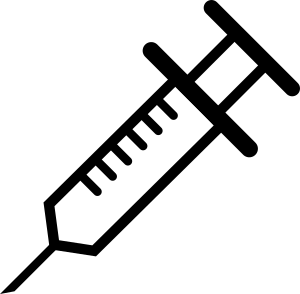
\includegraphics[width=1cm]{stock/syringe} };
    \end{tikzpicture}
    }
  \end{columns}

  \begin{columns}
    \column{0.33\textwidth}
    \uncover<2->{
    \centerline{\large predict}
    }

    \column{0.33\textwidth}
    \uncover<3->{
    \centerline{\large characterize}
    }

    \column{0.33\textwidth}
    \uncover<4->{
    \centerline{\large simulate}
    }
  \end{columns}
\end{frame}
